\section{Background}

\todo[inline]{Section introduction}

\subsection{Control Flow}

EBA provides a representation of the control flow of the input source files which is utilized in order to detect bugs. EBA generates a tree structure of the input, modeling statements as so-called \texttt{step}s. A path in this tree structure models a possible execution path, with each \texttt{step} in a path containing information about the modelled statements. The concrete tree structure modeling the resulting effects of statements can be formalized as a finite state machine $(\sum, S, s_0, \delta, F)$ as follows where $\sum$ is the input alphabet, $S$ is a finite non-empty set of states, $s_0$ is an element of $S$ and initial state, $\delta$ is the state-transition function $\delta: S \times \sum \rightarrow S$ and $F$ is the possibly empty set of final states and a subset of $S$. 

\begin{itemize}
    \item{
        $
            \begin{aligned}[t] 
                \sum = & \{\mathit{Entry}, \mathit{Nil}, (alloc, \rho), (free, \rho), (read, \rho), \\ & (write, \rho), (uninit, \rho), (call, \rho), (lock, \rho), (unlock, \rho)\}
            \end{aligned} 
        $
    }
    \item{
        $
            \begin{aligned}[t]
                S = & \{(allocated, \rho), (freed, \rho), (read, \rho), (written, \rho),\\ & (uninitialized, \rho), (called, \rho), (locked, \rho), (unlocked, \rho), End\}
            \end{aligned}
        $
    }
\end{itemize}

\noindent The remainder of the automaton definition is defined according to the control flow being modelled, where the initial state, $s_0$, is dependent on the control flow being modelled and therefore is an element of $\sum$. This also applies to the transition function $\delta$ and the set of final states $F$, which is also a subset of $\sum$. A concrete definition of an example control flow is shown below with an accompanying illustration of this in figure \ref{cfg_example-automaton}.

\begin{figure}[H]
    \centering
    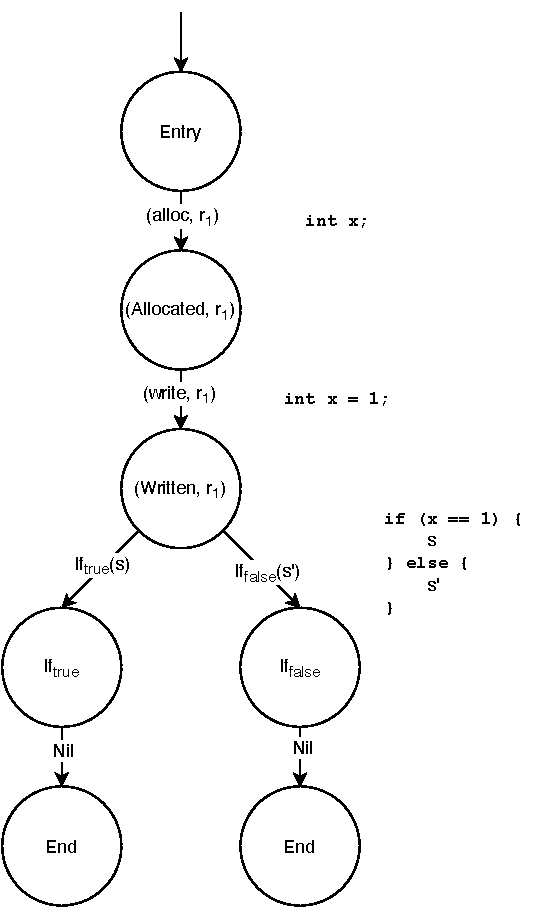
\includegraphics[width=0.5\textwidth]{background/figures/cfg_example}
    \caption{An illustration of a Control Flow automaton.}
    \label{cfg_example-automaton}
\end{figure}

\begin{itemize}
    \item $s_0 = Entry$ 
    \item {
        $
            \begin{aligned}[t]
            \delta = \text{the relation} \; \{ \; & (Entry, (\texttt{alloc},\rho), (allocated, \rho)), \\ 
            & (allocated, (\texttt{alloc},\rho), (allocated, \rho)), \\ 
            & ((allocated, \rho), (\texttt{lock}, \rho), (locked, \rho)), \\
            & ((locked, \rho), (\texttt{unlock}, \rho), (unlocked, \rho)), \\
            & ((unlocked, \rho), \texttt{unlock}, (unlocked, \rho), \\ 
            & ((write, \rho), \texttt{write}, (written, \rho)), \\ 
            & ((unlocked, \rho), \texttt{Nil}, End), \\ 
            & ((written, \rho), \texttt{Nil}, End) \; \}
            \end{aligned}
        $ 
    }
    \item $F = End$  
\end{itemize}

\noindent A few things are of note here; $Nil$ indicates the end of a path in the tree structure. Branches occur when an if-branch is encountered in the input source file and models the effects of the statements within if-statements.

\subsection{Monitor Templates}

\noindent \todo[inline]{How should the template generation function be defined?}

\noindent A monitor template is defined as the quintuple $X(\rho) \rightarrow (\sum, S, s_0, \delta, F)$ or \todo{Which one? Different one?} $X_\rho (\sum, S, s_0, \delta, F)$ where $\sum$ is the input alphabet, $S$ is a finite non-empty set of states happening on the region $\rho$, $s_0$ is an element of $S$ and initial state, $\delta$ is the state-transition function $\delta: S \times \sum \rightarrow S$ and $F$ is the possibly empty set of final states and a subset of $S$.

\newpar Monitor automata operate on the set of possible effects of a statement in the Control-flow Graph, which are defined as $E = \{$\texttt{alloc}, \texttt{free}, \texttt{read}, \texttt{write}, \texttt{uninit}, \texttt{call}, \texttt{lock}, \texttt{unlock}$\}$ by Abal \cite{EffectiveBugFinding}, corresponding all possible variants of the $mem\_kind$ type defined previously. 

\newpar Monitor automata in this thesis all operate on a subset of $E$ and have a non-empty set of final states, $F$, indicating that a possible bug is discovered.  

\subsubsection{Double-unlock monitor automata}

Given a region $\rho$, a double-unlock monitor automata is defined as the quintuple $(\sum, S, s_0, \delta, F)$ where: 

\begin{itemize}
    \item $\sum = \{\texttt{unlock}_\rho, \texttt{lock}_\rho\}$, a subset of $E$
    \item $S = \{ locked_\rho, unlocked_\rho, error_\rho \}$
    \item $s_0 = unlocked_\rho$ 
    \item $\delta =$ the relation $\{(locked_\rho, \texttt{unlock}_\rho, unlocked_\rho), (locked_\rho, \texttt{lock}_\rho, locked_\rho), \\
        (unlocked_\rho, \texttt{lock}_\rho, locked_\rho), (unlocked_\rho, \texttt{unlock}_\rho, error_\rho)\}$ 
    \item $F = error_\rho$  
\end{itemize}

An illustration of this monitor automata can be seen in figure \ref{double-unlock-automata}. 

\begin{figure}[H]
    \centering
    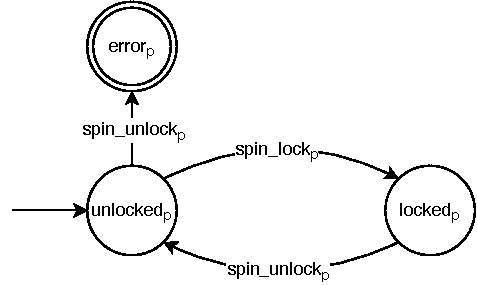
\includegraphics[width=0.5\textwidth]{background/figures/double-unlock}
    \caption{An illustration of a double-unlock monitor automata.}
    \label{double-unlock-automata}
\end{figure}

\newpar To show the detection of a possible double-unlock bug where a double-unlock monitor automaton has reached the final state, we find the product of the control flow example shown in figure \ref{cfg_example-automaton} and the monitor generated from the template. 

\begin{itemize}
    \item{
        $
            \begin{aligned}[t] 
                \sum = & \{\mathit{Entry}, \mathit{Nil}, (alloc, \rho), (free, \rho), (read, \rho), \\ 
                & (write, \rho), (uninit, \rho), (call, \rho), (lock, \rho), (unlock, \rho)\}
            \end{aligned} 
        $
    }
    \item{
        $
            \begin{aligned}[t]
                S = & \{(allocated, \rho), (freed, \rho), (read, \rho), (written, \rho),\\ 
                & (uninitialized, \rho), (called, \rho), \\
                & ((locked, \rho), locked_\rho), ((unlocked, \rho), unlocked_\rho), \\
                & ((unlocked, \rho), error_\rho), \\
                & End\}
            \end{aligned}
        $
    }
    \item $s_0 = Entry$ 
    \item {
        $
            \begin{aligned}[t]
            \delta = \text{the relation} \; \{ \; & (Entry, (\texttt{alloc},\rho), (allocated, \rho)), \\ 
            & (allocated, (\texttt{alloc},\rho), (allocated, \rho)), \\ 
            & ((allocated, \rho), (\texttt{lock}, \rho), (locked, \rho)), \\
            & ((locked, \rho), (\texttt{unlock}, \rho), ((unlocked, \rho), unlocked_\rho), \\
            & (((unlocked, \rho), unlocked_\rho), \texttt{unlock}, ((unlocked, \rho), error_\rho)), \\ 
            & (((write, \rho), unlocked_\rho), \texttt{write}, ((written, \rho), unlocked_\rho)), \\ 
            & (((unlocked, \rho), error_\rho), \texttt{Nil}, (End, error_\rho)), \\ 
            & (((written, \rho), unlocked_\rho), \texttt{Nil}, (End, error_\rho)) \; \}
            \end{aligned}
        $ 
    }
    \item $F = (End, error_\rho)$  
\end{itemize}

\noindent This product can be illustrated as follows. 

\begin{figure}[H]
    \centering
    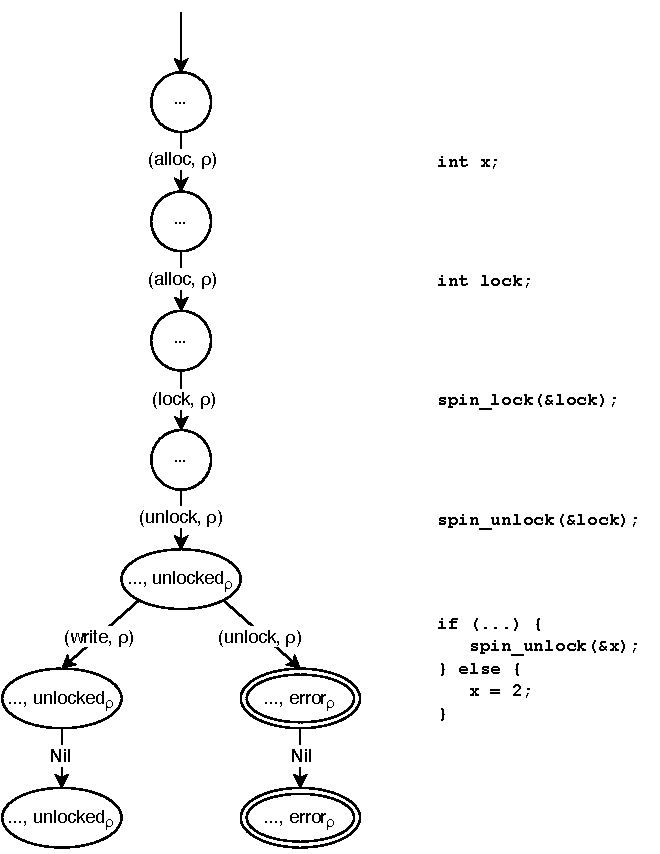
\includegraphics[width=0.5\textwidth]{background/figures/cfg_unlock-product}
    \caption{An illustration of the product construction of a double-unlock monitor automata and a control flow.}
    \label{cfg_unlock-product}
\end{figure}

\subsubsection{Double-lock monitor automata}

Given a region $\rho$, a double-lock monitor automata is defined as the quintuple $(\sum, S, s_0, \delta, F)$ where: 

\begin{itemize}
    \item $\sum = \{\texttt{lock}_\rho, \texttt{unlock}_\rho\}$, a subset of $E$
    \item $S = \{ locked_\rho, unlocked_\rho, error_\rho \}$
    \item $s_0 = unlocked_\rho$ 
    \item $\delta =$ the relation $\{(unlocked_\rho, \texttt{lock}_\rho, locked_\rho), (locked_\rho, \texttt{unlock}_\rho, unlocked_\rho), \\
    (locked_\rho, \texttt{lock}_\rho, error_\rho), (unlocked_\rho, \texttt{unlock}_\rho, unlocked_\rho)\}$ 
    \item $F = error_\rho$  
\end{itemize}

An illustration of this monitor automata can be seen in figure \ref{double-lock-automata}. 

\begin{figure}[H]
    \centering
    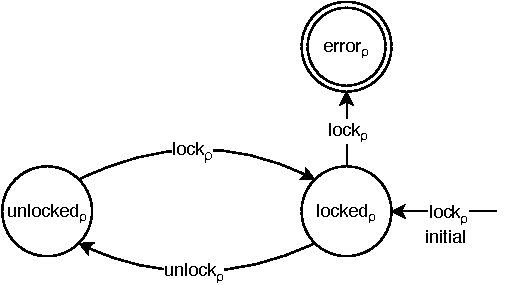
\includegraphics[width=0.5\textwidth]{background/figures/double-lock}
    \caption{An illustration of a double-lock monitor automata.}
    \label{double-lock-automata}
\end{figure}

\subsubsection{Double-free monitor automata}

Given a region $\rho$, a double-free monitor automata is defined as the quintuple $(\sum, S, s_0, \delta, F)$ where: 

\begin{itemize}
    \item $\sum = \{\texttt{free}_\rho, \texttt{alloc}_\rho\}$, a subset of $E$
    \item $S = \{ allocated_\rho, freed_\rho, error_\rho \}$
    \item $s_0 = freed_\rho$ 
    \item $\delta =$ the relation $\{(freed_\rho, \texttt{alloc}_\rho, allocated_\rho), (allocated_\rho, \texttt{free}_\rho, freed_\rho), \\
    (freed_\rho, \texttt{free}_\rho, error_\rho), (allocated_\rho, \texttt{alloc}_\rho, allocated_\rho)\}$ 
    \item $F = error_\rho$  
\end{itemize}

An illustration of this monitor automata can be seen in figure \ref{double-free-automata}. 

\begin{figure}[H]
    \centering
    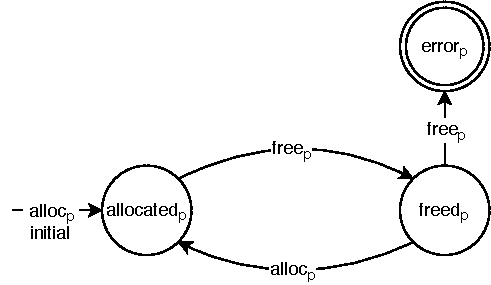
\includegraphics[width=0.5\textwidth]{background/figures/double-free}
    \caption{An illustration of a double-free monitor automata.}
    \label{double-free-automata}
\end{figure}

\subsubsection{Use-before-init monitor automata}

Given a region $\rho$, a use-before-init monitor automata is defined as the quintuple $(\sum, S, s_0, \delta, F)$ where: 

\begin{itemize}
    \item $\sum = \{\texttt{read}_\rho, \texttt{init}_\rho\}$, a subset of $E$
    \item $S = \{ unread_\rho, initialized_\rho, error_\rho \}$
    \item $s_0 = unused_\rho$ 
    \item $\delta =$ the relation $\{(unread_\rho, \texttt{init}_\rho, initialized_\rho), (initialized_\rho, \texttt{uninit}_\rho, unread_\rho), \\
    (unread_\rho, \texttt{read}_\rho, error_\rho), (initialized_\rho, \texttt{init}_\rho, initialized_\rho)\}$ 
    \item $F = error_\rho$  
\end{itemize}

An illustration of this monitor automata can be seen in figure \ref{use-before-automata}. 

\begin{figure}[H]
    \centering
    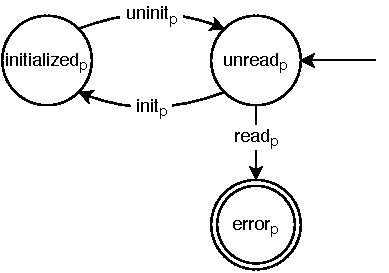
\includegraphics[width=0.5\textwidth]{background/figures/use-before}
    \caption{An illustration of a use-before-init monitor automata.}
    \label{use-before-automata}
\end{figure}